\documentclass[aspectratio=169, table, 12pt]{beamer}

\usepackage{colortbl}
\usepackage{xcolor}
\usepackage{listings}
\usepackage{tabularx}
\usepackage{tikz}
\usetikzlibrary{arrows.meta, positioning, calc, fit, shapes.geometric}

\makeatletter
\def\input@path{{../theme/}}
\makeatother
\graphicspath{{../theme/}{../../figures/}}
\usetheme{Pradita}

\definecolor{praditagreen}{RGB}{37, 113, 71}

% Tema membuat garis tabel berwarna putih. Dikembalikan agar tabel terbaca.
\arrayrulecolor{black}
\setlength{\arrayrulewidth}{0.5pt}

% Kolom X rata kiri, dipakai pada tabel dengan kolom X yang sempit, agar
% spasi antarkata tidak meregang.
\newcolumntype{Y}{>{\raggedright\arraybackslash}X}

\lstdefinelanguage{bash}{
  keywords={},
  basicstyle=\ttfamily\scriptsize,
  ndkeywords={cd, coverage, curl, diff, docker, echo, npm, npx, python,
              python3, pytest, source},
  ndkeywordstyle=\color{purple}\bfseries,
  sensitive=true,
  commentstyle=\color{gray},
  numbers=none,
  breaklines=true,
  frame=lines,
  backgroundcolor=\color{lightgray!10},
  tabsize=2,
  comment=[l]{\#},
  showstringspaces=false
}

\lstdefinelanguage{TypeScript}{
  keywords={const, let, function, return, async, await, try, catch, throw,
            new, if, interface, void, export, import, from, type},
  ndkeywords={Promise, number, string, boolean, test, expect, Page, await},
  basicstyle=\ttfamily\scriptsize,
  keywordstyle=\color{blue}\bfseries,
  ndkeywordstyle=\color{purple}\bfseries,
  sensitive=true,
  commentstyle=\color{gray}\itshape,
  stringstyle=\color{red},
  numbers=none,
  breaklines=true,
  frame=lines,
  backgroundcolor=\color{lightgray!10},
  tabsize=2,
  comment=[l]{//},
  morestring=[b]",
  showstringspaces=false
}

% Gaya Python disamakan dengan naskah bab, tanpa nomor baris.
\lstdefinestyle{PythonStyle}{
  language=Python,
  basicstyle=\ttfamily\scriptsize,
  morekeywords={with, as, yield, async, await, match, case},
  keywordstyle=\color{blue}\bfseries,
  emph={pytest, psycopg, Mock, given, strategies},
  emphstyle=\color{purple}\bfseries,
  commentstyle=\color{gray}\itshape,
  stringstyle=\color{red},
  numbers=none,
  breaklines=true,
  frame=lines,
  backgroundcolor=\color{lightgray!10},
  tabsize=2,
  showstringspaces=false
}

% File mutu dan kontrak ditampilkan apa adanya, sehingga butuh gaya JSON.
\lstdefinelanguage{json}{
  basicstyle=\ttfamily\scriptsize,
  stringstyle=\color{red},
  commentstyle=\color{gray},
  numbers=none,
  breaklines=true,
  frame=lines,
  backgroundcolor=\color{lightgray!10},
  tabsize=2,
  showstringspaces=false,
  morestring=[b]"
}

\title{\Huge Testing, Reliability,\\ \vspace{10pt} dan Code Quality}
\subtitle{IF140303 - Pengembangan Aplikasi Web}
\author{\textbf{Alfa Yohannis}}

\begin{document}

\frame{\titlepage}

\begin{frame}[fragile]
  \frametitle{Isi Pertemuan}
  \vspace{14pt}
  \begin{columns}[t]
    \column{0.5\textwidth}
    {\small\tableofcontents[sections={1-7}]}

    \column{0.5\textwidth}
    {\small\tableofcontents[sections={8-14}]}
  \end{columns}
\end{frame}

\begin{frame}{\hfill}
  \centering
  \Huge{\textbf{Apakah kodenya masih benar\\sesudah diubah?}}
\end{frame}

\section{Tujuan dan Kerangka Bahasan}

\begin{frame}{\hfill}
  \centering
  \Huge{\textbf{Tujuan dan Kerangka Bahasan}}
\end{frame}

\begin{frame}{{\Large Tujuan Pembelajaran}}
  \vspace{10pt}
  \begin{itemize}
    \item Membedakan unit test, integration test, dan End-to-End (E2E) test
          berdasarkan biaya waktunya dan jenis cacat yang tertangkap
          masing-masing.
    \item Merancang \textit{test double} dan pengujian kontrak untuk
          memisahkan bagian yang diuji dari layanan lain, lalu membuktikannya
          lewat pengujian yang berjalan tanpa layanan itu menyala.
    \item Mengukur mutu kode lewat \textit{coverage}, analisis statis, dan
          jumlah \textit{query} per alamat, lalu menegakkannya sebagai
          \textit{quality gate} yang memblokir \textit{merge}.
  \end{itemize}
\end{frame}

\begin{frame}{{\Large Yang Belum Dijawab Bab 5}}
  \vspace{12pt}
  \begin{itemize}
    \item Bab 5 menutup pertanyaan cepat atau lambat dengan angka.
    \item Yang belum dijawab lebih mendasar: apakah kodenya masih benar
          sesudah diubah.
    \item Mencoba sendiri di browser berhenti bekerja begitu jumlah alamat
          bertambah, karena tidak ada yang sanggup mencoba seluruhnya pada
          tiap perubahan.
  \end{itemize}
  \vspace{8pt}
  {\small Seluruh angka pada pertemuan ini diukur dari aplikasi pesanan di
  \texttt{sources/chapter06}.}
\end{frame}

\section{Tiga Lapisan Pengujian}

\begin{frame}{\hfill}
  \centering
  \Huge{\textbf{Tiga Lapisan Pengujian}}
\end{frame}

\begin{frame}{{\Large Apa Bedanya}}
  \vspace{12pt}
  \begin{itemize}
    \item \textbf{Unit test} menguji satu bagian kecil, tanpa menyentuh apa
          pun di luarnya.
    \item \textbf{Integration test} menguji beberapa bagian yang bekerja
          bersama, termasuk basis data sungguhan.
    \item \textbf{E2E test} menjalankan aplikasinya seperti pengguna, lewat
          browser, dan memeriksa apa yang tergambar di layar.
  \end{itemize}
  \vspace{8pt}
  {\small Analoginya memeriksa sepeda: memutar pedal di tempat, memasang
  rantai lalu memutarnya, atau mengayuhnya keliling lapangan.}
\end{frame}

\begin{frame}{{\Large Harga Tiap Lapisan}}
  \vspace{6pt}
  \centering
  {\footnotesize
  \begin{tabularx}{\textwidth}{lrrY}
    \hline
    \textbf{Lapisan} & \textbf{Jumlah} & \textbf{Waktu} & \textbf{Yang tertangkap} \\
    \hline
    Unit & 19 & 0,43 s & Salah hitung, salah batas, salah syarat \\
    \hline
    Integrasi dan kontrak & 15 & 0,91 s & Salah \textit{query}, bentuk \textit{response} berubah \\
    \hline
    E2E lewat Chrome & 5 & 2,00 s & Tombol tak terhubung, modul gagal dimuat \\
    \hline
  \end{tabularx}}

  \vspace{8pt}
  {\small Satu pengujian E2E memakan waktu lebih lama daripada seluruh 19
  unit test digabung. Karena itu jumlah tiap lapisan tidak dibuat sama.}
\end{frame}

\begin{frame}{{\Large Piramida lawan Trophy}}
  \vspace{4pt}
  \centering
  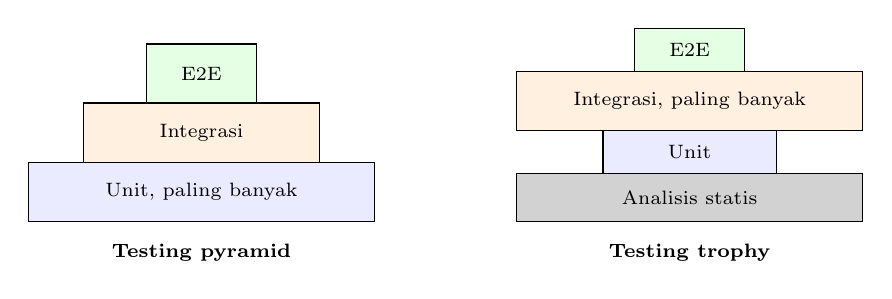
\begin{tikzpicture}[font=\scriptsize]
    \fill[blue!8, draw=black] (0,0) rectangle (4.4,0.75);
    \node at (2.2,0.375) {Unit, paling banyak};
    \fill[orange!12, draw=black] (0.7,0.75) rectangle (3.7,1.5);
    \node at (2.2,1.125) {Integrasi};
    \fill[green!10, draw=black] (1.5,1.5) rectangle (2.9,2.25);
    \node at (2.2,1.875) {E2E};
    \node[font=\scriptsize\bfseries] at (2.2,-0.4) {Testing pyramid};

    \fill[gray!35, draw=black] (6.2,0) rectangle (10.6,0.6);
    \node at (8.4,0.3) {Analisis statis};
    \fill[blue!8, draw=black] (7.3,0.6) rectangle (9.5,1.15);
    \node at (8.4,0.875) {Unit};
    \fill[orange!12, draw=black] (6.2,1.15) rectangle (10.6,1.9);
    \node at (8.4,1.525) {Integrasi, paling banyak};
    \fill[green!10, draw=black] (7.7,1.9) rectangle (9.1,2.45);
    \node at (8.4,2.175) {E2E};
    \node[font=\scriptsize\bfseries] at (8.4,-0.4) {Testing trophy};
  \end{tikzpicture}

  \vspace{8pt}
  {\small Piramida lahir ketika integration test masih mahal dan rapuh.
  \textit{Trophy} lahir sesudah container membuat basis data sungguhan
  menyala dalam hitungan detik.}
\end{frame}

\section{Test Double}

\begin{frame}{\hfill}
  \centering
  \Huge{\textbf{Test Double}}
\end{frame}

\begin{frame}{{\Large Empat Jenis Pengganti}}
  \vspace{6pt}
  \centering
  {\footnotesize
  \begin{tabularx}{\textwidth}{lYl}
    \hline
    \textbf{Jenis} & \textbf{Menjawab pertanyaan} & \textbf{Di Bab 6} \\
    \hline
    Dummy & Tidak menjawab apa pun, hanya mengisi argumen wajib & \texttt{Mock()} kosong \\
    \hline
    Stub & Apa hasilnya bila layanan menjawab nilai tertentu & \texttt{StubBiayaKirim} \\
    \hline
    Fake & Apakah aturannya benar untuk banyak masukan & \texttt{FakeBiayaKirim} \\
    \hline
    Mock & Apakah layanannya dipanggil, dan dengan argumen apa & \texttt{Mock()} + \texttt{assert} \\
    \hline
  \end{tabularx}}

  \vspace{8pt}
  {\small Namanya diambil dari \textit{stunt double} di film: pemeran
  pengganti untuk adegan yang tidak perlu dikerjakan pemeran aslinya.}
\end{frame}

\begin{frame}[fragile]{{\Large Mock Membuktikan Panggilan yang Tidak Terjadi}}
  \vspace{2pt}
\begin{lstlisting}[style=PythonStyle]
def test_mock_membuktikan_layanan_tidak_dipanggil():
  mock_klien = Mock()
  ongkir = layanan_kirim.hitung_ongkir(mock_klien, KODE_POS_JAKARTA,
                                       BERAT_GRAM, gratis_ongkir=True)
  assert ongkir == 0
  mock_klien.minta_biaya.assert_not_called()
\end{lstlisting}
  \vspace{4pt}
  {\small Yang diperiksa bukan hasil hitungannya, melainkan ada atau tidaknya
  panggilan. Sifat itu tidak dapat dibuktikan dari nilai kembalian.}
\end{frame}

\begin{frame}{{\Large Kapan Diganti, Kapan Tidak}}
  \vspace{14pt}
  \begin{itemize}
    \item Bagian milik sendiri diuji apa adanya.
    \item Bagian milik orang lain diganti.
  \end{itemize}
  \vspace{10pt}
  {\small Karena itu layanan biaya kirim diganti, sedangkan PostgreSQL tetap
  dipakai sungguhan: perilaku basis datanya justru yang ingin dibuktikan.}
\end{frame}

\section{Basis Data di Container}

\begin{frame}{\hfill}
  \centering
  \Huge{\textbf{Basis Data di Container}}
\end{frame}

\begin{frame}{{\Large Mengapa Bukan Tiruan}}
  \vspace{12pt}
  \begin{itemize}
    \item Cacat yang paling sering lolos lahir dari perbedaan antara tiruan
          dan basis data aslinya.
    \item Contohnya tipe \texttt{numeric} yang tidak dikenal \texttt{json},
          atau urutan baris yang berbeda ketika \texttt{ORDER BY} lupa
          ditulis.
  \end{itemize}
  \vspace{10pt}
  {\small Masalahnya satu: pengujian yang menulis akan mengotori data uji,
  sehingga pengujian berikutnya bergantung pada urutan.}
\end{frame}

\begin{frame}[fragile]{{\Large Transaksi yang Selalu Dibatalkan}}
  \vspace{2pt}
\begin{lstlisting}[style=PythonStyle]
@pytest.fixture()
def koneksi():
  """Memberi satu koneksi basis data yang dibatalkan sesudah pengujian.

  Rollback membuat pengujian dapat menulis tanpa mengotori data uji, sehingga
  urutan pengujian tidak lagi menentukan hasilnya.
  """
  with basis_data.buka_koneksi() as koneksi_uji:
    yield koneksi_uji
    koneksi_uji.rollback()
\end{lstlisting}
  \vspace{2pt}
  {\small Dua akibatnya: pengujian boleh ditulis dalam urutan apa pun, dan
  data uji tidak perlu dibangun ulang antarpengujian.}
\end{frame}

\section{Contract Testing}

\begin{frame}{\hfill}
  \centering
  \Huge{\textbf{Pengujian API\\dan Contract Testing}}
\end{frame}

\begin{frame}{{\Large Memeriksa Bentuk, Bukan Isi}}
  \vspace{12pt}
  \begin{itemize}
    \item Yang dijaga adalah janji yang dipegang klien: nama field, tipenya,
          dan field mana yang selalu ada.
    \item Janji itu ditulis sebagai JSON Schema di
          \texttt{kontrak/pesanan.schema.json}, lalu dipakai pengujian untuk
          memeriksa server.
  \end{itemize}
  \vspace{10pt}
  {\small Menambah satu field lolos dari integration test, karena nilai yang
  diperiksanya tidak berubah. Kontraknya menyala, karena
  \texttt{additionalProperties} bernilai \texttt{false}.}
\end{frame}

\begin{frame}{{\Large Yang Diperiksa Kontrak}}
  \vspace{6pt}
  \centering
  {\footnotesize
  \begin{tabularx}{\textwidth}{lY}
    \hline
    \textbf{Yang diperiksa} & \textbf{Janjinya} \\
    \hline
    Status 200 & Bentuk \textit{response} cocok skema, tanpa field tambahan \\
    \hline
    Tipe field & \texttt{id} dan \texttt{total} bilangan bulat, \texttt{status} salah satu dari empat nilai \\
    \hline
    Status 400 & Id bukan angka ditolak tanpa menyentuh basis data \\
    \hline
    Status 404 & Id yang tidak ada dijawab 404, bukan 500 \\
    \hline
    Header & \texttt{X-Query-Count} selalu ada dan berisi angka \\
    \hline
  \end{tabularx}}
\end{frame}

\section{Property-Based Testing}

\begin{frame}{\hfill}
  \centering
  \Huge{\textbf{Property-Based Testing}}
\end{frame}

\begin{frame}[fragile]{{\Large Sifat, Bukan Contoh}}
  \vspace{2pt}
\begin{lstlisting}[style=PythonStyle]
@given(jumlah_unit=UNIT, harga_satuan=HARGA_SATUAN)
def test_diskon_tidak_melebihi_subtotal(jumlah_unit, harga_satuan):
  """Potongan selalu lebih kecil daripada belanjanya, sehingga tidak gratis."""
  subtotal = harga.hitung_subtotal(jumlah_unit, harga_satuan)
  assert 0 <= harga.hitung_diskon(jumlah_unit, subtotal) <= subtotal
\end{lstlisting}
  \vspace{4pt}
  {\small Unit test biasa hanya memeriksa contoh yang terpikirkan penulisnya.
  Di sini yang ditulis adalah sifat yang harus selalu benar, lalu pustakanya
  yang mencari angka pembantahnya dan menyusutkannya menjadi contoh terkecil
  yang masih gagal.}
\end{frame}

\section{Coverage dan Analisis Statis}

\begin{frame}{\hfill}
  \centering
  \Huge{\textbf{Coverage\\dan Analisis Statis}}
\end{frame}

\begin{frame}{{\Large Dua Suite, Coverage Sama}}
  \vspace{6pt}
  \centering
  {\footnotesize
  \begin{tabularx}{\textwidth}{Yrr}
    \hline
    \textbf{Suite yang dijalankan} & \textbf{Pengujian} & \textbf{Coverage} \\
    \hline
    Seluruh \texttt{test\_harga.py} & 10 & 100\% \\
    \hline
    Tanpa pengujian batas, \texttt{-k "not batas\_grosir"} & 9 & 100\% \\
    \hline
  \end{tabularx}}

  \vspace{8pt}
  {\small \texttt{harga.py} berisi 23 pernyataan, dan kedua suite
  menyentuh seluruhnya. Perbedaannya baru terlihat ketika kodenya dirusak
  dengan sengaja.}
\end{frame}

\begin{frame}{{\Large Mutasi: >= Menjadi >}}
  \vspace{6pt}
  \centering
  {\footnotesize
  \begin{tabularx}{\textwidth}{Yll}
    \hline
    \textbf{Suite yang dijalankan} & \textbf{Coverage} & \textbf{Hasil} \\
    \hline
    Tanpa pengujian batas & 100\% & 9 lolos, mutasi tidak tertangkap \\
    \hline
    Seluruh pengujian & 100\% & 1 gagal, mutasi tertangkap \\
    \hline
  \end{tabularx}}

  \vspace{8pt}
  {\small \textit{Coverage} menjawab baris mana yang dijalankan, bukan apakah
  hasilnya diperiksa. Pesanan tepat sepuluh unit adalah satu-satunya contoh
  yang membedakan kedua tanda banding.}
\end{frame}

\begin{frame}{{\Large Analisis Statis}}
  \vspace{14pt}
  \begin{itemize}
    \item Membaca kode tanpa menjalankannya, lalu melaporkan hal yang
          mencurigakan: nama yang tidak dipakai, \textit{import} menggantung,
          perbandingan yang selalu benar.
    \item Alatnya \texttt{ruff}, dan hasilnya nol temuan pada seluruh file
          sumber Bab 6.
  \end{itemize}
  \vspace{10pt}
  {\small Inilah alas \textit{testing trophy}: sebagian cacat tertangkap
  sebelum satu pengujian pun berjalan.}
\end{frame}

\section{Quality Gate di CI}

\begin{frame}{\hfill}
  \centering
  \Huge{\textbf{Quality Gate di CI}}
\end{frame}

\begin{frame}{{\Large Tempat Gate Bekerja}}
  \vspace{14pt}
  \centering
  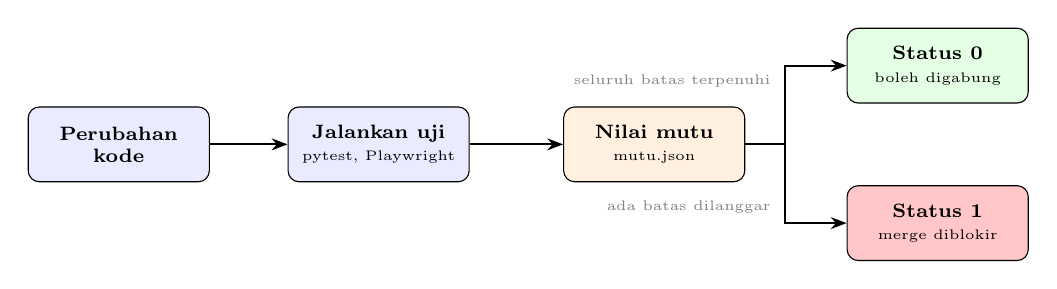
\begin{tikzpicture}[
    font=\scriptsize,
    kotak/.style={draw, rounded corners, minimum height=0.95cm,
                  minimum width=2.3cm, align=center, font=\scriptsize\bfseries},
    panah/.style={-{Stealth[length=2mm]}, thick}
  ]
    \node[kotak, fill=blue!8] (ubah) at (0,0) {Perubahan\\kode};
    \node[kotak, fill=blue!8] (uji) at (3.3,0) {Jalankan uji\\{\tiny\mdseries pytest, Playwright}};
    \node[kotak, fill=orange!12] (nilai) at (6.8,0) {Nilai mutu\\{\tiny\mdseries mutu.json}};
    \node[kotak, fill=green!10] (gabung) at (10.4,1.0) {Status 0\\{\tiny\mdseries boleh digabung}};
    \node[kotak, fill=red!22] (tolak) at (10.4,-1.0) {Status 1\\{\tiny\mdseries merge diblokir}};

    \draw[panah] (ubah) -- (uji);
    \draw[panah] (uji) -- (nilai);
    \draw[panah] (nilai.east) -- ++(0.5,0) |- (gabung.west);
    \draw[panah] (nilai.east) -- ++(0.5,0) |- (tolak.west);
    \node[font=\tiny, gray, anchor=east] at (8.4,0.8) {seluruh batas terpenuhi};
    \node[font=\tiny, gray, anchor=east] at (8.4,-0.8) {ada batas dilanggar};
  \end{tikzpicture}

  \vspace{12pt}
  {\small Batasnya ditulis di \texttt{mutu.json}: waktu tiap lapisan,
  \textit{coverage} minimum, temuan analisis statis, dan jumlah
  \textit{query} tiap alamat.}
\end{frame}

\begin{frame}[fragile]{{\Large Penutup Gate}}
  \vspace{2pt}
\begin{lstlisting}[style=PythonStyle]
  jumlah_langgar = sum(1 for baris in daftar_baris if not baris[-1])
  if jumlah_langgar:
    print(f"\nGagal: {jumlah_langgar} batas mutu dilanggar.")
    sys.exit(1)
  print("\nLolos: seluruh batas mutu terpenuhi.")
\end{lstlisting}
  \vspace{4pt}
  {\small \textit{Continuous Integration} membaca status keluarnya, bukan
  tulisan di layar. Satu perintah \texttt{python gate-mutu.py} di dalam
  \textit{pipeline} sudah cukup untuk memblokir \textit{merge}.}
\end{frame}

\begin{frame}[fragile]{{\Large Membaca Verdict Gate}}
  \vspace{2pt}
\begin{lstlisting}[language=bash]
python gate-mutu.py

# Keluarannya:
#   Pemeriksaan                             Batas            Terukur  Verdict
#   pytest unit                                 0                 0   lolos
#   waktu unit                                 10 s           0.83 s  lolos
#   pytest integrasi                            0                 0   lolos
#   waktu integrasi                            30 s            1.3 s  lolos
#   coverage harga.py                          95 %            100 %  lolos
#   temuan ruff                                 0                 0   lolos
#   query /api/pesanan/1                        2                 2   lolos
#   query /api/pesanan-n1/1                     2                 5   LANGGAR
#
# Gagal: 1 batas mutu dilanggar.
\end{lstlisting}
\end{frame}

\begin{frame}{{\Large Cacat yang Tidak Terlihat dari Response}}
  \vspace{12pt}
  \begin{itemize}
    \item Alamat \texttt{/api/pesanan-n1/1} memberi \textit{response} yang
          sama persis dengan alamat sehat.
    \item Seluruh pengujian isinya hijau.
    \item Yang membedakan hanya jumlah \textit{query}, yaitu 5 lawan 2 untuk
          pesanan berisi tiga item.
  \end{itemize}
  \vspace{8pt}
  {\small Cacat seperti itu hanya tertangkap karena jumlahnya ikut diukur dan
  dilaporkan lewat header \texttt{X-Query-Count}.}
\end{frame}

\section{Persiapan Latihan}

\begin{frame}{\hfill}
  \centering
  \Huge{\textbf{Persiapan Latihan}}
\end{frame}

\begin{frame}[fragile]{{\Large Basis Data, Venv, dan Dependensi}}
  \vspace{2pt}
\begin{lstlisting}[language=bash]
cd sources/chapter06
docker compose up -d
./siapkan-data.sh
python3 -m venv ../.venv
../.venv/bin/pip install "psycopg[binary]" pytest hypothesis jsonschema \
  coverage ruff
npm install
\end{lstlisting}
  \vspace{2pt}
  {\small Dilakukan sekali. Basis datanya di port 5436, aplikasinya di port
  8020, dan browsernya memakai Google Chrome yang sudah terpasang lewat
  channel \texttt{chrome}.}
\end{frame}

\section{Latihan 1: Tiga Lapisan}

\begin{frame}{\hfill}
  \centering
  \Huge{\textbf{Latihan 1\\Membandingkan Tiga Lapisan}}
\end{frame}

\begin{frame}{{\Large Langkah Kerja}}
  \vspace{8pt}
  \begin{enumerate}
    \item Jalankan ketiga lapisan, lalu catat jumlah pengujian dan waktunya.
    \item Hitung berapa kali lipat satu pengujian E2E dibandingkan rata-rata
          satu unit test.
    \item Matikan aplikasinya, jalankan ulang lapisan E2E, dan catat apa yang
          terjadi. Nyalakan kembali sesudahnya.
  \end{enumerate}
  \vspace{8pt}
  {\small Latihan ini membuktikan ketiga lapisan berbeda harganya, dan
  menangkap cacat yang berbeda pula.}
\end{frame}

\begin{frame}[fragile]{{\Large Menjalankan Ketiganya}}
  \vspace{2pt}
\begin{lstlisting}[language=bash]
source ../.venv/bin/activate
pytest -q test_harga.py test_properti.py test_double.py
pytest -q test_integrasi.py test_kontrak.py
python aplikasi.py &
npx playwright test --config e2e/playwright.config.ts
\end{lstlisting}
\end{frame}

\begin{frame}{{\Large Contoh Hasil Latihan 1}}
  \vspace{6pt}
  \centering
  {\footnotesize
  \begin{tabularx}{\textwidth}{lrrY}
    \hline
    \textbf{Lapisan} & \textbf{Jumlah} & \textbf{Waktu} & \textbf{Catatan} \\
    \hline
    Unit & 19 & 0,43 s & Tanpa basis data dan tanpa jaringan \\
    \hline
    Integrasi dan kontrak & 15 & 0,91 s & Basis data di container \\
    \hline
    E2E & 5 & 2,00 s & Chrome sungguhan, satu \textit{worker} \\
    \hline
  \end{tabularx}}
\end{frame}

\begin{frame}{{\Large Lembar Isian Latihan 1}}
  \vspace{4pt}
  \centering
  {\footnotesize
  \begin{tabularx}{\textwidth}{lrrY}
    \hline
    \textbf{Lapisan} & \textbf{Jumlah} & \textbf{Waktu} & \textbf{Catatan} \\
    \hline
    Unit & \dots & \dots & \dots \\
    \hline
    Integrasi dan kontrak & \dots & \dots & \dots \\
    \hline
    E2E & \dots & \dots & \dots \\
    \hline
    E2E tanpa aplikasi menyala & \dots & \dots & \dots \\
    \hline
  \end{tabularx}}

  \vspace{6pt}
  {\footnotesize Pertanyaan: cacat apa yang hanya tertangkap lapisan E2E,
  mengapa unit test tetap dibuat paling banyak, dan apa akibatnya bila
  seluruh pengujian dipindahkan ke lapisan E2E?}
\end{frame}

\section{Latihan 2: Coverage yang Menipu}

\begin{frame}{\hfill}
  \centering
  \Huge{\textbf{Latihan 2\\Coverage yang Menipu}}
\end{frame}

\begin{frame}{{\Large Langkah Kerja}}
  \vspace{6pt}
  \begin{enumerate}
    \item Ukur \textit{coverage} \texttt{harga.py} untuk seluruh
          \texttt{test\_harga.py}, lalu ukur lagi tanpa pengujian batas.
    \item Ubah \texttt{>=} menjadi \texttt{>} pada \texttt{hitung\_diskon}.
          Ini disebut mutasi.
    \item Jalankan kedua suite terhadap kode yang sudah dimutasi, lalu catat
          mana yang lolos dan mana yang gagal.
    \item Kembalikan \texttt{harga.py} seperti semula, lalu pastikan seluruh
          pengujian kembali hijau.
  \end{enumerate}
\end{frame}

\begin{frame}[fragile]{{\Large Mengukur Dua Kali}}
  \vspace{2pt}
\begin{lstlisting}[language=bash]
source ../.venv/bin/activate
coverage run -m pytest -q test_harga.py
coverage report --include="harga.py"
coverage run -m pytest -q test_harga.py -k "not batas_grosir"
coverage report --include="harga.py"

# Keluarannya:
# Name       Stmts   Miss  Cover
# harga.py      23      0   100%
\end{lstlisting}
\end{frame}

\begin{frame}{{\Large Contoh Hasil Latihan 2}}
  \vspace{6pt}
  \centering
  {\footnotesize
  \begin{tabularx}{\textwidth}{Yllr}
    \hline
    \textbf{Suite} & \textbf{Coverage} & \textbf{Sesudah mutasi} & \textbf{Gagal} \\
    \hline
    Seluruh \texttt{test\_harga.py} & 100\% & tertangkap & 1 \\
    \hline
    Tanpa pengujian batas & 100\% & lolos & 0 \\
    \hline
  \end{tabularx}}
\end{frame}

\begin{frame}{{\Large Lembar Isian Latihan 2}}
  \vspace{4pt}
  \centering
  {\footnotesize
  \begin{tabularx}{\textwidth}{Yllr}
    \hline
    \textbf{Suite} & \textbf{Coverage} & \textbf{Sesudah mutasi} & \textbf{Gagal} \\
    \hline
    Seluruh \texttt{test\_harga.py} & \dots & \dots & \dots \\
    \hline
    Tanpa pengujian batas & \dots & \dots & \dots \\
    \hline
    Mutasi pilihan sendiri & \dots & \dots & \dots \\
    \hline
  \end{tabularx}}

  \vspace{6pt}
  {\footnotesize Pertanyaan: mengapa \textit{coverage} tetap 100 persen
  padahal satu pengujian dibuang, dan pengujian seperti apa yang perlu
  ditambahkan agar mutasi semacam ini selalu tertangkap?}
\end{frame}

\section{Latihan 3: Menangkap N+1}

\begin{frame}{\hfill}
  \centering
  \Huge{\textbf{Latihan 3\\Menangkap N+1 Lewat Query}}
\end{frame}

\begin{frame}{{\Large Langkah Kerja}}
  \vspace{6pt}
  \begin{enumerate}
    \item Nyalakan aplikasinya, lalu panggil kedua alamat dengan
          \texttt{curl} dan catat header \texttt{X-Query-Count}.
    \item Hitung berapa item yang dimiliki pesanan itu, lalu cocokkan dengan
          rumus dua ditambah jumlah item.
    \item Bandingkan isi kedua \textit{response} dengan \texttt{diff}.
    \item Ulangi untuk satu pesanan lain yang jumlah itemnya berbeda.
  \end{enumerate}
\end{frame}

\begin{frame}[fragile]{{\Large Membaca Jumlah Query}}
  \vspace{2pt}
\begin{lstlisting}[language=bash]
curl -s -D - -o sehat.json http://127.0.0.1:8020/api/pesanan/1 \
  | grep -i x-query-count
curl -s -D - -o n1.json http://127.0.0.1:8020/api/pesanan-n1/1 \
  | grep -i x-query-count
diff sehat.json n1.json && echo "isi response sama persis"

# Keluarannya:
# X-Query-Count: 2
# X-Query-Count: 5
# isi response sama persis
\end{lstlisting}
\end{frame}

\begin{frame}{{\Large Contoh Hasil dan Lembar Isian Latihan 3}}
  \vspace{4pt}
  \centering
  {\footnotesize
  \begin{tabularx}{\textwidth}{lrrrY}
    \hline
    \textbf{Pesanan} & \textbf{Item} & \textbf{Query sehat} & \textbf{Query N+1} & \textbf{Isi response} \\
    \hline
    1 & 3 & 2 & 5 & sama persis \\
    \hline
  \end{tabularx}}

  \vspace{6pt}
  \centering
  {\footnotesize
  \begin{tabularx}{\textwidth}{lrrrY}
    \hline
    \textbf{Pesanan} & \textbf{Item} & \textbf{Query sehat} & \textbf{Query N+1} & \textbf{Isi response} \\
    \hline
    1 & \dots & \dots & \dots & \dots \\
    \hline
    Pesanan pilihan sendiri & \dots & \dots & \dots & \dots \\
    \hline
  \end{tabularx}}

  \vspace{4pt}
  {\footnotesize Pertanyaan: mengapa pengujian yang hanya membandingkan isi
  tidak menangkap cacat ini, dan mengapa jumlah \textit{query} lebih layak
  dijadikan batas daripada waktu jalannya?}
\end{frame}

\section{Latihan 4: Quality Gate}

\begin{frame}{\hfill}
  \centering
  \Huge{\textbf{Latihan 4\\Menegakkan Quality Gate}}
\end{frame}

\begin{frame}{{\Large Langkah Kerja}}
  \vspace{6pt}
  \begin{enumerate}
    \item Baca \texttt{mutu.json}, lalu tulis dugaan pemeriksaan mana yang
          akan dilanggar dan mengapa.
    \item Jalankan gerbangnya, catat \textit{verdict} tiap baris beserta
          status keluarnya.
    \item Longgarkan batas \textit{query} alamat N+1 menjadi tiga puluh, lalu
          jalankan ulang dan catat status keluarnya.
    \item Kembalikan batasnya menjadi dua, perbaiki cacatnya dengan
          mengarahkan halaman demo ke alamat yang sehat, lalu jalankan ulang.
  \end{enumerate}
\end{frame}

\begin{frame}{{\Large Contoh Hasil Latihan 4}}
  \vspace{6pt}
  \centering
  {\footnotesize
  \begin{tabularx}{\textwidth}{Yllr}
    \hline
    \textbf{Pemeriksaan} & \textbf{Batas} & \textbf{Terukur} & \textbf{Verdict} \\
    \hline
    waktu unit & 10 s & 0,83 s & lolos \\
    \hline
    coverage \texttt{harga.py} & 95\% & 100\% & lolos \\
    \hline
    temuan \texttt{ruff} & 0 & 0 & lolos \\
    \hline
    query \texttt{/api/pesanan-n1/1} & 2 & 5 & LANGGAR \\
    \hline
    Status keluar & 0 & 1 & LANGGAR \\
    \hline
  \end{tabularx}}
\end{frame}

\begin{frame}{{\Large Lembar Isian Latihan 4}}
  \vspace{4pt}
  \centering
  {\footnotesize
  \begin{tabularx}{\textwidth}{Yllr}
    \hline
    \textbf{Pemeriksaan} & \textbf{Batas} & \textbf{Terukur} & \textbf{Verdict} \\
    \hline
    waktu unit & \dots & \dots & \dots \\
    \hline
    waktu integrasi & \dots & \dots & \dots \\
    \hline
    coverage \texttt{harga.py} & \dots & \dots & \dots \\
    \hline
    temuan \texttt{ruff} & \dots & \dots & \dots \\
    \hline
    query \texttt{/api/pesanan/1} & \dots & \dots & \dots \\
    \hline
    query \texttt{/api/pesanan-n1/1} & \dots & \dots & \dots \\
    \hline
    Status keluar sebelum dan sesudah dilonggarkan & \dots & \dots & \dots \\
    \hline
  \end{tabularx}}
\end{frame}

\begin{frame}[fragile]{{\Large Membersihkan}}
  \vspace{2pt}
\begin{lstlisting}[language=bash]
docker compose down -v
\end{lstlisting}
  \vspace{6pt}
  {\small Opsi \texttt{-v} ikut menghapus volume datanya, sehingga penyiapan
  berikutnya dimulai dari keadaan bersih.}
\end{frame}

\section{Ringkasan}

\begin{frame}{\hfill}
  \centering
  \Huge{\textbf{Ringkasan}}
\end{frame}

\begin{frame}{{\Large Ringkasan}}
  \vspace{8pt}
  \begin{itemize}
    \item Tiga lapisan, tiga harga: 19 unit test 0,43 detik, 15 pengujian
          integrasi dan kontrak 0,91 detik, 5 pengujian E2E 2,00 detik.
    \item Bagian milik orang lain diganti \textit{test double}, bagian milik
          sendiri diuji apa adanya. Basis datanya sungguhan, dan tiap
          pengujian dibungkus transaksi yang dibatalkan.
    \item Kontrak menjaga bentuk \textit{response}, sedangkan integration
          test menjaga isinya.
    \item \textit{Coverage} 100 persen pada dua suite yang berbeda, tetapi
          hanya satu yang menangkap mutasi \texttt{>=} menjadi \texttt{>}.
    \item Gerbang mutu menilai waktu, \textit{coverage}, temuan
          \texttt{ruff}, dan jumlah \textit{query}, lalu keluar dengan status
          1 begitu satu batas dilanggar.
  \end{itemize}
\end{frame}

\end{document}
